\section{Introduction}
\label{sec:eval_intro}
In this chapter, detail experiment settings, executions and results are discussed.
Section~\ref{sec:eval_setdetail} details hardware configurations and data set we use. 
There are 5 experiments conducted. In Section~\ref{sec:eval_diffval}, we discuss the experiment 
where we assess runtime to access object's field with different variable types. 
Section~\ref{sec:eval_refcount} shows details to examine how behaviors of normal reference and Reference Count are different. 
Section~\ref{sec:eval_sort} describes our Merge-sort experiment to examine behavior of Atomic Reference Counting.
Two algorithms are discussed used in Big Data processing and examined in our experiments: 
Tree-aggregate in Section~\ref{sec:concept_treeagg} and K-Nearest-Neighbors in Section~\ref{sec:concept_knn}.

\section{Experimental Set and Detail}
\label{sec:eval_setdetail}
We have used two different data sets. One is a real-world data set, Wikipedia page data set,
and another is a syntactic randomized generated data set based on Complex object described in Section~\ref{sec:concept_compobj}. 
We use one machine with particular specification.
\subsection{Wikipedia Data Sets}
 \label{sec:concept_dataset}
 Wikipedia page data sets are used to perform document classification with KNN. 
 We have separated the data set into training and test data set, 
 \(10^5\) pages are used for training data set, and 18724 pages are used for target.

 \subsection{Experimental Details}
 \label{sec:concept_expdetail}
 All experiments are run on VM instances on Google Cloud Platform, 
 n1-standard-8 which has 8 vCPU, 30 GB RAM, and 10 GB Standard persistent disk.
 In this thesis, we present the result of runtime as the average of 5 separate runs for each experiment.

\section{Experiment 1: Accessing Object with Different Variable Type}
\label{sec:eval_diffval}
This experiment is conducted to understand two questions. One is how different variable types have impact to runtime performance.
The other is how initialization of Vec size has impact to runtime performance. 
In this experiment, we focus on owner, reference, and slice as a variable of sequence values. 
Since these variables have different memory representation, there might be differences among time for access to actual values of each variables.

To evaluate this assumption, we use the three types of complex object: CustomerOwned, CustomerBorrowed and CustomerSlice. 
At first, we generate source Vecs for all fields, Vecs which contain all elements used for corresponding fields of objects.
For example, all of i32 elements used for key field in 1 million Customer object are stored in Vec$<$i32$>$ with 1 million i32 elements. 
Later, these i32 elements are moved to be owned or borrowed by the object's fields.

Next, 1.5, 1.8, 2.5, 2.8, 3.5, and 3.8 million of Customer objects are created and stored in Vec. 
When a Customer Vec is created, whether size of Vec is initialized is controlled. 
Finally, serialization of Customer object is performed as an operation forcing program to access all of fields in the object.
This serialization is performed each Customer objects in the Vec. We measure total runtime to serialize all of Customer objects 
stored in Vec. 

\subsection{Result}
\label{sec:history}
The result is shown in Figure~\ref{fig:rustaccessinit} and Figure~\ref{fig:rustaccessnoinit}.
Figure~\ref{fig:rustaccessinit} is comparison of the runtime performance among different Customer object types with Vec size initialization.
Figure~\ref{fig:rustaccessnoinit} is comparison in the same set of experiment except Vec size is not initialized. 
The blue, yellow, and green chats represent runtime of access to fields of CustomerOwned, CustomerBorrowed, and CustomerSlice objects respectively.

No matter Vec size initialized or not, differences of runtime for accessing objects are not remarkable among different object types. 
The percent increase in runtime of accessing to fields of from 1.5 to 3.8 million CustomerOwned objects is 121\% if the Vec is initialized, 554\% if the Vec is not initialized.

Considering the differences of percent increase of runtime whether the Vec is initialized or not, 
Figure\ref{fig:init_vs_noinit} the comparison of runtime access to fields of CustomerOwned object with and without Vec Initialization.
For 3.8 million of objects, the difference of runtime to access to the objects is 38745 secounds; program without Vec initialization is 60\% slower than one with the initialization.

\begin{figure}[htb]
    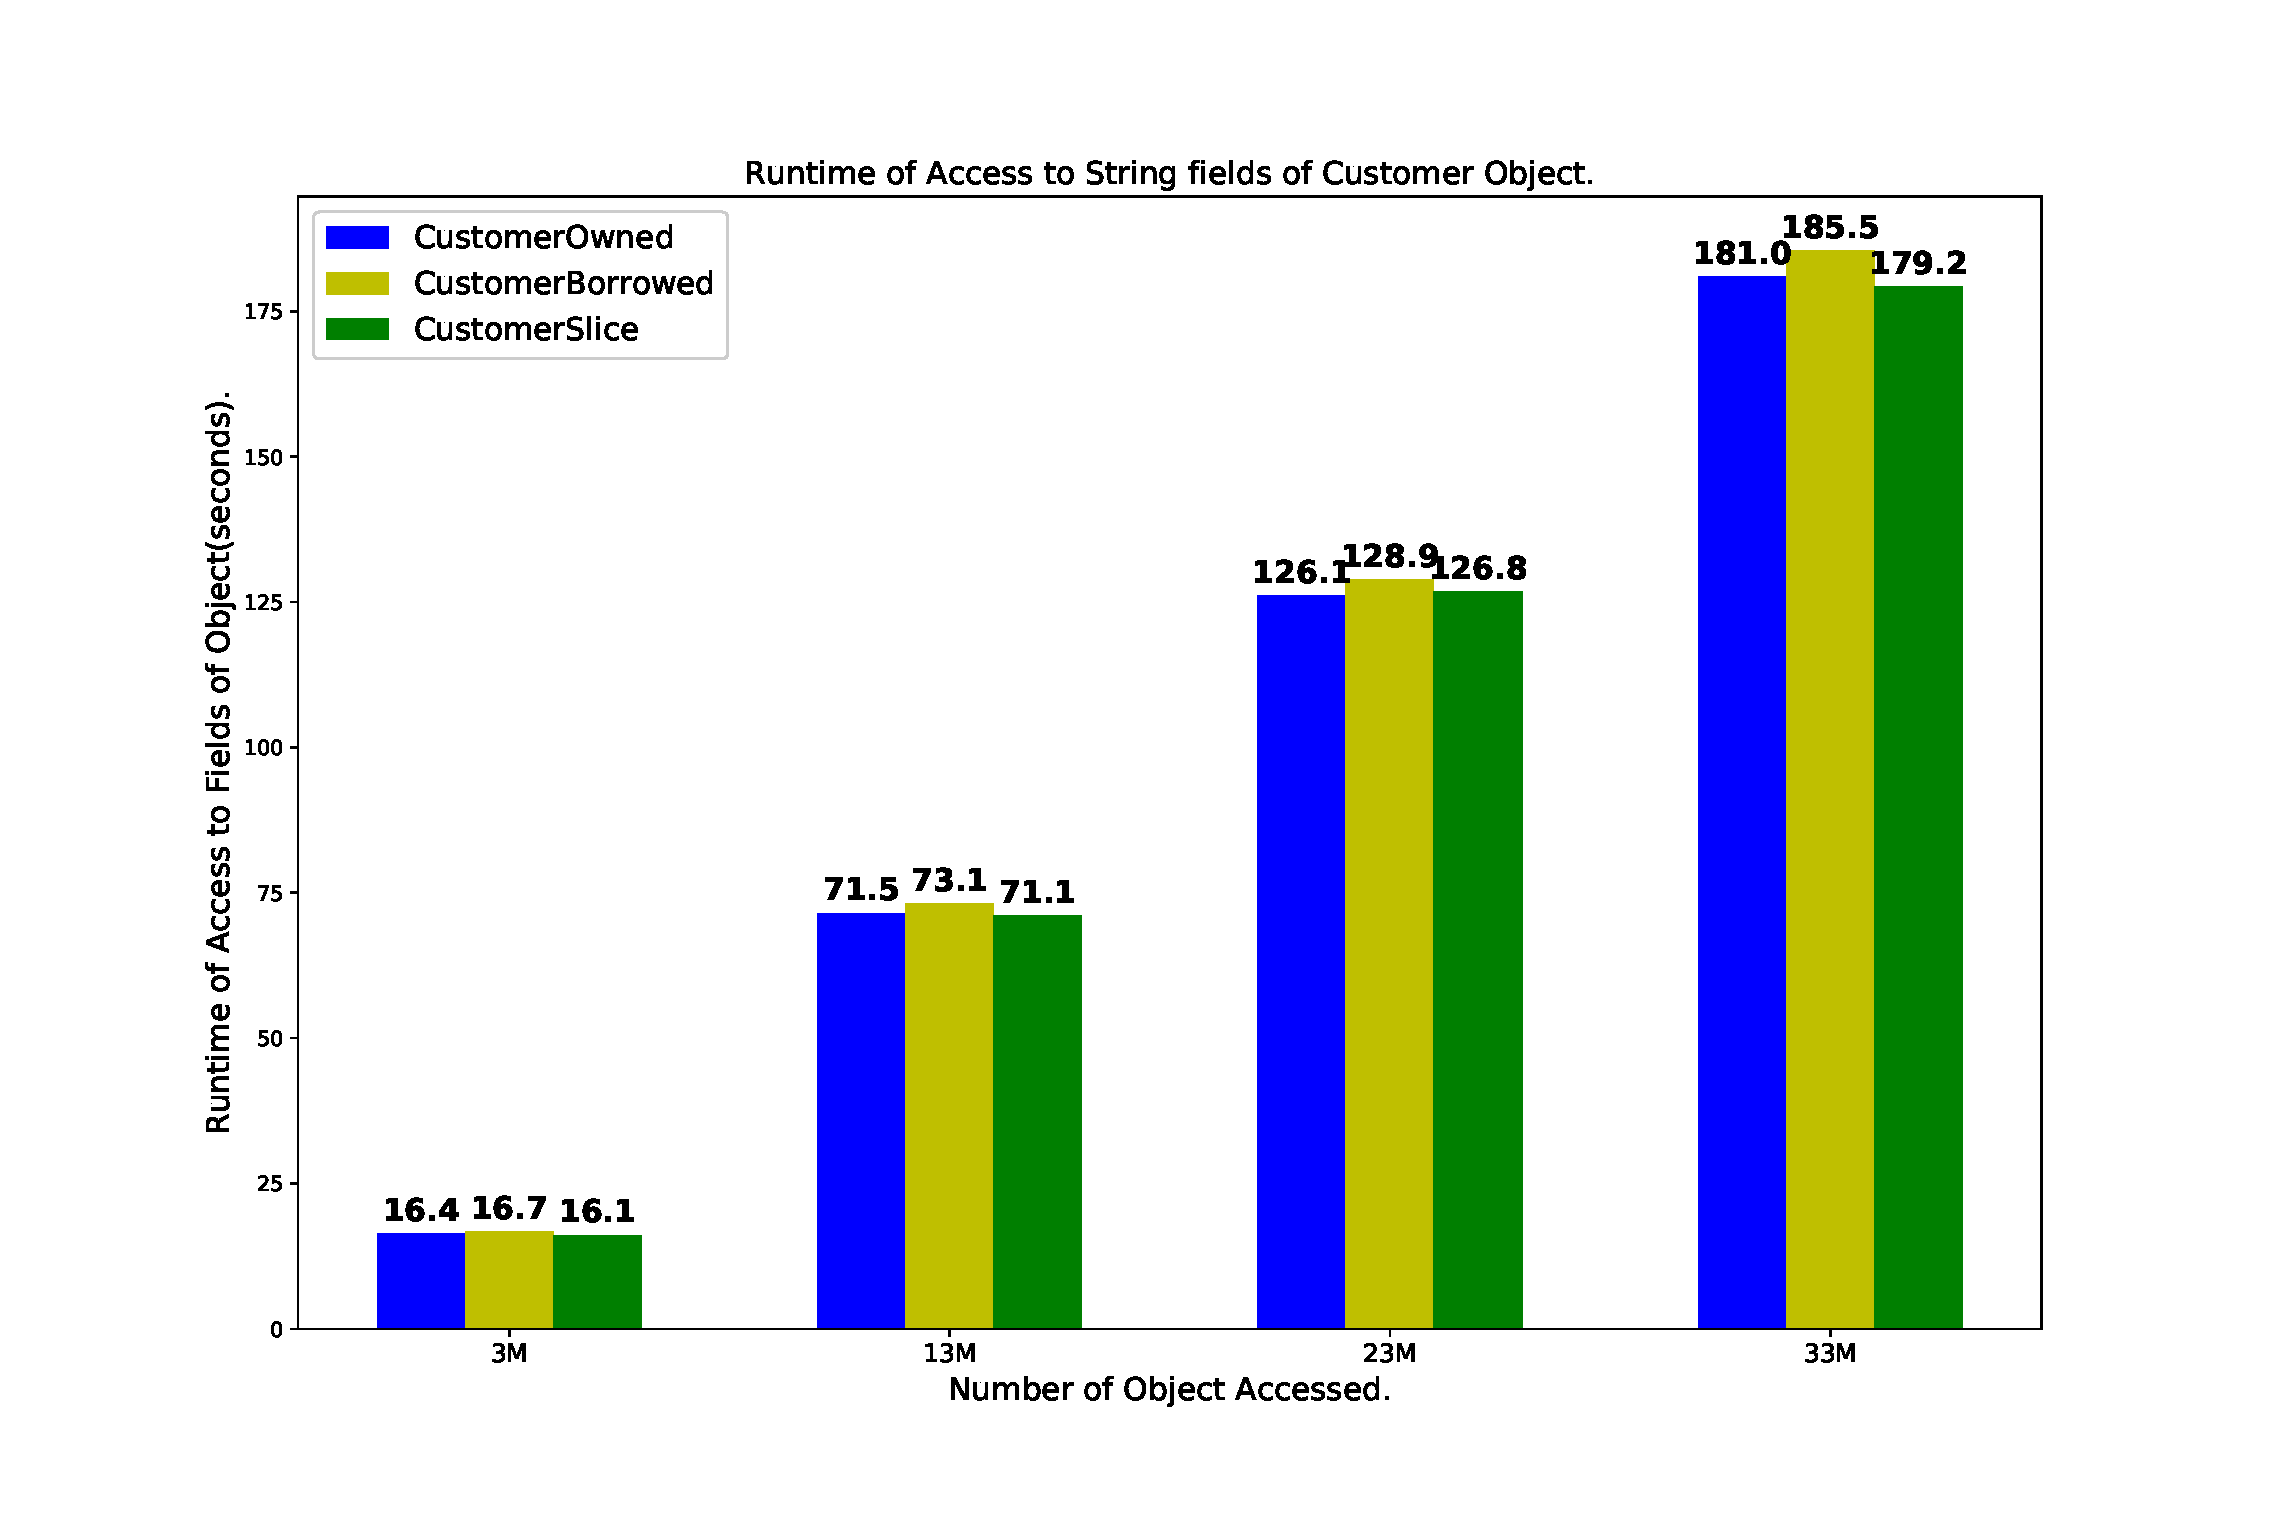
\includegraphics[width=15cm]{rust_access_different_poniter_init.eps}
    \caption{Runtime of Access to Different Pointer Types with Vec Size Initialization}
    \label{fig:rustaccessinit}
\end{figure}

\begin{figure}[htb]
    \includegraphics[width=15cm]{rust_access_different_poniter_noinit.eps}
    \caption{Runtime of Access to Different Pointer Types without Vec Size Initialization}
    \label{fig:rustaccessnoinit}
\end{figure}

\begin{figure}[htb]
    \includegraphics[width=15cm]{rust_access_init_vs_noint.eps}
    \caption{Runtime of Access to Fields of Complex Object with Initialization vs without Initialization}
    \label{fig:init_vs_noinit}
\end{figure}

\subsection{Discussion}
\label{sec:history}
Difference of variable types does not have huge impact to runtime of accessing to actual value.
Even thought owner, reference , and slice have different memory representations, the access time to its value is 
close to each other. As shown in Figure~\ref{fig:own_ref_slice}, the representations of owner and slice are almost identical except slice does not have capacity for values.
Reference is pointer pointing to owner, so it has an additional step to access actual value. 
However, the result shows this additional step does not have huge impact for runtime to access memory region of the value.

Whether initializing Vec size results in disparity of runtime performance to access objects' fields. 
This is because when Vec uninitialized, the elements of Vec are allocated across different virtual memory pages.



\section{Experiment 2: Assessment of different reference methods in Rust}
\label{sec:eval_refcount}
\subsection{Concept}
The goal of this experiment is to assess efficiency of different reference strategies in Rust, borrowing and reference counting. 

By levaraging reference counting, a value can be shared like what borrowing plays the role in Rust programming. 
The difference is that reference counting checks number of reference pointing to the actual data and makes sure the data is not deleted 
until all the references are dereferenced. Using reference counting is sometimes preferable approach for developers, 
we do not have care about lifetime which is usually troublesome when we use borrowing approach many times in our code. 
However, the possible problem regarding to reference counting is the cost for tracking the number of references. 
Having this assumption, this experiment will show difference of behavior among reference countinig and borrowing.

In this experiment, CustomerBorrowed and CustomerRc in figure are used to see difference of dropping time among borrowing and reference counting. 
In the CustomerRc and OrderRc struct, all fields take reference counting (Rc$<$T$>$). Similaly to the experiment in the last section, 
vectors of CustomerRc and CustomerBorrowed are created and droped the elements one by one. 

The result shows significant difference of dropping time among the two objects; deletion of CustomerRc is much slower than CustomerBorrowed. 
This is because reference counters which are feilds of CustomerRc have to check the number of reference pointing to the actual content and decide 
deallocate the memory or not. However, memory management and lifetime strategy of borrowing is already determined at compile time.


In this experiment, an assessment is conducted to valify whether there is difference between behavior of borrowing and reference counting. 
These two methods can be used in similar situation. Especially, when we want reference to an original variable and keep the original variable until all of references are dereferenced, 
we can have reference with both storategies, borrowing and reference counting. One advantage of using reference counting is that we do not have to pay attention to lifetime.
However, the assumption here is that use of reference counting might be computationally expenesive than borrowing, because reference counting has to track the number of reference pointing to the value. 
Considered this assumption, we assess difference of time for dropping reference using borrowing and reference counting strategies. 

Similally to the last section, we implement struct whose fields are borrowing reference and reference counting and measure the time to drop the struct. 


\subsection{Result}
The result shows the time to drop borrowing reference is significatly faster than reference counting. This says that we should use borrwoing storategies whenever high performance computation is critical.
\begin{figure}[htb!]
    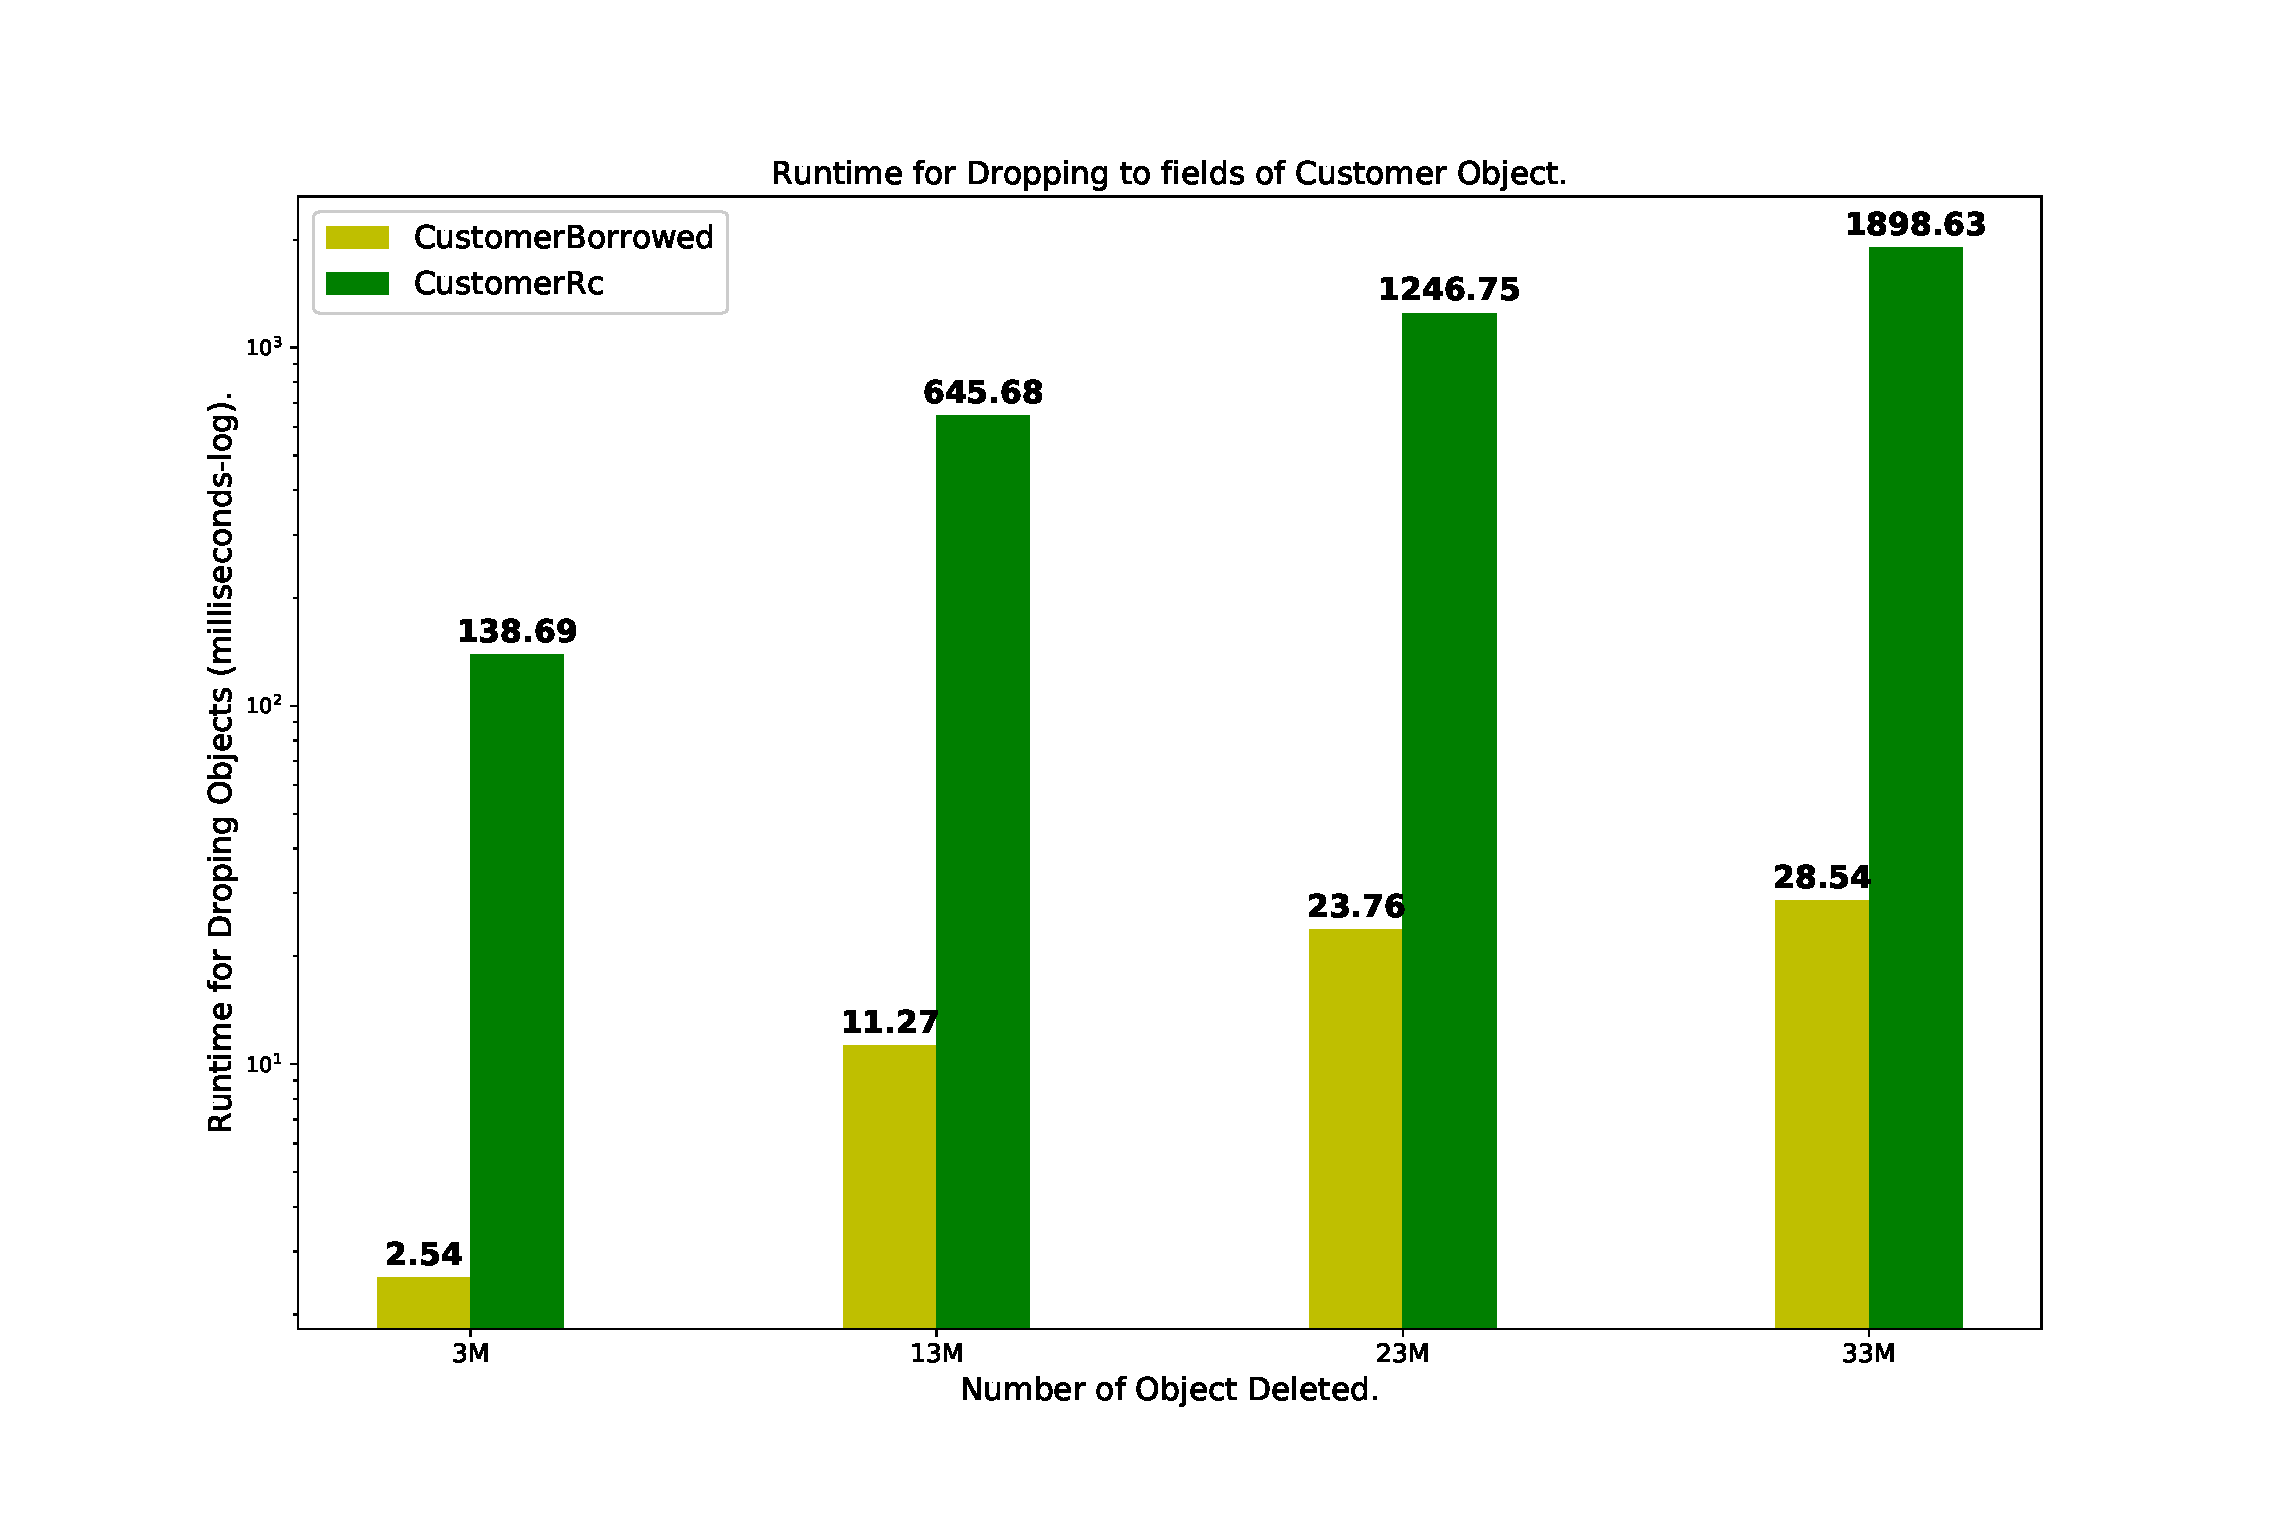
\includegraphics[width=15cm]{rust_droptime_borring_rc.eps}
    \caption{Runtime for Droping to fields of Customer Object}
    \label{fig:Sampling}
\end{figure}

\subsection{Discussion}


\section{Experiment 3: Merge-sort}
\label{sec:eval_sort}
This experiment is to assess importance of careful memory management in multithreading of Rust. 
We implement merge-sort algorithm in two different ways. One is sharing source vector with Arc. 
The other is passing slice of source vector to child thread. 

Our merge-sort algorithm with vector is implemented with recursion. In these alogorithm, the splitting phase is merely aquiring index of split position, 
not actually splitting the source vector. At merge phase, merge function receives two independent vector and merge these into single new vector.

For sharing data implementaion, channel with sending data is used for multithreading method, because we want to ensure children threads return values before parent thread proceed execution. 
For passing slice implementation, we use scope method to enable children threads to receive reference from their parent ensuring the same purpose of sending data. 

Experiment performed is the comparison among sharing data and passing slice implementations to see the impact of Arc, Atomic reference conuting, to runtime performance.
These two implementations are theoritically the same operations other than using or not using Arc to share data. 
This comparison can effectively show how important careful memory management is in multithreading computation in Rust. 
In another word, how atomic reference counting can cost for computation in Rust programming.

The figure shows the result of 
An atomic reference count of the shareable vector is passed to every recursion steps and 


\begin{figure}[htb]
    \includegraphics[width=15cm]{rust_merge_sort.eps}
    \caption{Runtime of Sortting Elements of Customer Vector}
    \label{fig:Sampling}
\end{figure}



The other is LinkedList implementation other than vector.
The linkedlist implementation is different from another two. This algorithm is inplace sorting so that it does not de/allocate memory during execution. 
The comparison among vector and linkedlist implementations can show trade-off between contiguous memory access and inplace non memory de/allocation. 
Experiment with Java linkedlist implementation can be interesting, because Java GC is severe problem when number of object is large. 


\section{Experiment 4: Tree-aggregation}
\label{sec:eval_treeagg}
Tree-aggregate is a communication patten heavily used for Machine Learning algorithm in Spark (MLlib). 
In the traditional aggregation function in Spark, results of aggregation in all executor clusters are sent to the driver. 
That is why this operation suffers from the CUP cost in merging partial results and the network bandwidth limit.
Tree-aggregate is a communication pattern which overcomes these problems by breaking aggregate operation in multi-level represented like tree structure.

In multi-thread situation, tree-aggregate is just fork-join thread algorithm. We already implemented Merge-Sort algorithm with fork-join. 
If we implement tree-aggregate with multi-thread, the difference is only aggregation and sorting.

\section{Experiment 5: K-Nearest-Neighbors}
\label{sec:eval_knn}
Finally, we examine performance of a Machine Learning (ML) algorithms. 
The goal of this experiment is to evaluate better memory management strategies in ML algorithms developed with Rust.
We employ K-Nearest-Neighbors (KNN) for ML algorithm to be studied in our experiments.
Our KNN algorithms perform document classification on Wikipedia page data set described in Section~\ref{sec:eval_setdetail}. 

The algorithms have 4 phase; load, preprocess, query, and combine phase. 
The algorithms spawn threads at the beginning ,and in the load phase partition of files are loaded in each threads. 
In preprocessing phase, the algorithm process document strings to generate Term-frequencies (Tfs) matrices and other data structures. 
In query phase, it calculates cosine similarities between all combination of train and test observations and select to top \(K\) nearest neighbors. 
In combine phase, the results from each batch and from each are combined. 
Based on our experiments result, the runtime in preprocess and query phase are significantly larger than other two phases.
Therefore, we focus discussion in these two phases considering them bottlenecks in our KNN algorithms.

KNN algorithms are implemented with different memory management strategies. 
We parametrize these memory management and some other values. These parameters are listed in Table~\ref{tab:parameter}. 

\begin{table}
    \renewcommand{\arraystretch}{1.2}
    \begin{tabular}{|l|l|l|l|l|}
    \hline
    Parameter Name  & \multicolumn{4}{l|}{Values and Description}                                                                                                                                                                                \\ \hline
    Method          & \multicolumn{4}{l|}{\begin{tabular}[c]{@{}l@{}}deep-copy:  use deep-copy to generate intermediate objects\\ arc: use atomic reference count to generate intermediate objects\end{tabular}}                                 \\ \hline
    Strategy        & \multicolumn{4}{l|}{\begin{tabular}[c]{@{}l@{}}1: keep intermediate objects in memory until owner is changed\\ 2: remove intermediate objects as soon as it is not needed\end{tabular}}                                    \\ \hline
    Number of batch & \multicolumn{4}{l|}{\begin{tabular}[c]{@{}l@{}}2: generate 2 batch from each partition\\ 3: generate 3 batch from each partition\end{tabular}}                                                                             \\ \hline
    k               & \multicolumn{4}{l|}{\begin{tabular}[c]{@{}l@{}}15K: dimension of feature matrices is 15 thousands \\ 20K: dimension of feature matrices is 20 thousands\\ 25K: dimension of feature matrices is 25 thousands\end{tabular}} \\ \hline
    \end{tabular}
    \caption{Parameter of KNN algorithms}
    \label{tab:parameter}
 \end{table}


Method parameter is specified to select memory management strategy used in preprocess phase. 
In preprocess phase, the algorithm generates many intermediate data structures using same String elements.
Deep-copy method deeply copies String to generate intermediate data structures. Arc method use Atomic Reference Count (Arc) to wrap String elements in the original data structure and 
clone Arc when the elements are used in other data structures. As Experiment 4 had shown in in Section~\ref{sec:eval_treeagg}, deep-copy of complex objects is more expensive than cloning Arc. 
String is a sort of objects allocated in heap and copied many times in preprocess phase. Therefore, it is worth to assess which method can be better memory management strategy in our experiments.

Strategy parameter controls memory management strategy used in both preprocess and query phase.
Strategy 1 keeps all intermediate data structures and numeric matrix objects from preprocess to query phase. 
Strategy 2 removes these data structures and objects as soon as they are not needed. 
These strategies differ from each other in terms of memory usage and frequency of memory deallocations.
These may cause significant runtime difference of the algorithms.

Number of batch controls number and size of batch for each partition. This parameter varies size of intermediate data structures and numeric matrices, and 
frequency of memory deallocations. Parameter k specifies dimension of feature matrices. This determines size of intermediate data structures and numeric matrices.

By controlling these parameter, we compare runtime and memory usage of KNN algorithms. 


\subsection{Result}
\label{sec:history}
Figure~\ref{fig:total}, ~\ref{fig:preprocess}, and ~\ref{fig:query} show the runtime performance of our KNN algorithms in total, preprocess, and query phase respectively. 
The algorithms whose runtime is showing 0 seconds are algorithms that are terminated during execution due to fail of memory allocation.
The algorithm with 2 batches, strategy 1, Arc method, and 20K and 25K dimension, 
and the algorithm with 2 batches, strategy 1, deep-copy method, 25K dimension are such algorithms whose memory capacity get over during execution time.

As shown in Figure~\ref{fig:preprocess}, the algorithms using Arc is much slower than using deep-copy in preprocessing phase. 
If we set algorithm's parameter in 3 batches , strategy 2, and 25K dimension, the algorithm with Arc is about 38\% slower than the one with deep-copy. 
In addition, the algorithms with strategy 2 are slower than with strategy 1. When the parameters are set in 3 batches, deep-copy method, and 25K dimension, 
runtime performance of the algorithm with strategy 2 is about 85\% slower than one with strategy 1. 
Furthermore, as we increase the number of dimension, the number of batch becomes more and more critical to runtime performance of the algorithms with deep-copy.
The runtime differences among different number of batch are about 44\%, 28\%, and 39\% for the algorithms whose parameters are set in strategy 2 and Arc method. 
However, those for the algorithms with strategy 2 and deep-copy method are about 11\%, 28\%, and 54\%. The ratios of difference increase proportionally to the number of dimension. 



\begin{figure}[htb]
    \includegraphics[width=15cm]{total.eps}
    \caption{Total runtime whole KNN algorithm (seconds)}
    \label{fig:total}
\end{figure}

\begin{figure}[htb]
    \includegraphics[width=15cm]{preprocessing.eps}
    \caption{Total runtime of preprocessing phase in KNN (seconds)}
    \label{fig:preprocess}
\end{figure}


\begin{figure}[htb]
    \includegraphics[width=15cm]{query.eps}
    \caption{Total runtime of query phase in KNN (seconds)}
    \label{fig:query}
\end{figure}


\subsection{Discussion}
\label{sec:history}


\section{Summary}
\label{sec:eval_summary}
In this chapter, we examines various memory management strategies for different algorithms in Rust programming.
There are many factors that might differ performance of algorithms: different variable type, Reference Counting, Atomic Reference Counting, and frequency of memory de/allocation.
We should select the best memory management strategies when developing Big Data processing tools. 
Some of tips for the development are proved in our experiments. We conclude this thesis in Chapter~\ref{chapter:Conclusions}.

% \section{Elements Copy and Insertion into Size-initialized Vector in Rust.}
% \label{sec:history}
% In this experiment, four methods are used to insert elements into vector in Rust. One is clone method which performs bitwise deep copy. 
Another is clone\_from which also performs bitwise deep copy, but copies elements of the vector to distination vector rather than 
creating new one. We initialize the distination vector with the same size to the number of elements we insert into it. 
Another is copy\_nonoverlapping function which copies values from source to distination memory region. 
The other is pushing elements of source to distination vector one by one. Insertions of elements with 4 size are conducted 1000000, 1500000, 10000000, 15000000, and, 
their runtimes for each elements type, integer and String are measured. 


The figure shows the result of the experiment. Among the runtime performances of integer insertion for every methods, 
clone, clone\_from, and copy\_nonoverlapping method shows the similar performance. However, the pushing the copy of elements one by one has much slower runtime performance 
compared to the rest. This is because integer elements are allocated contiguously in the memory, so that accessing address of memory by pointer reads some next address. 
This boosts the copy and insertion of elements. 

On the other hand, all of methods show the similar runtime performance in experiment for String object insertion. 
This is because String object is not stored in contiguous memory region. The vector stores pointer to the object and 
process need to access around different memory region again and again to deeply copy the object.

\begin{figure}[htb]
    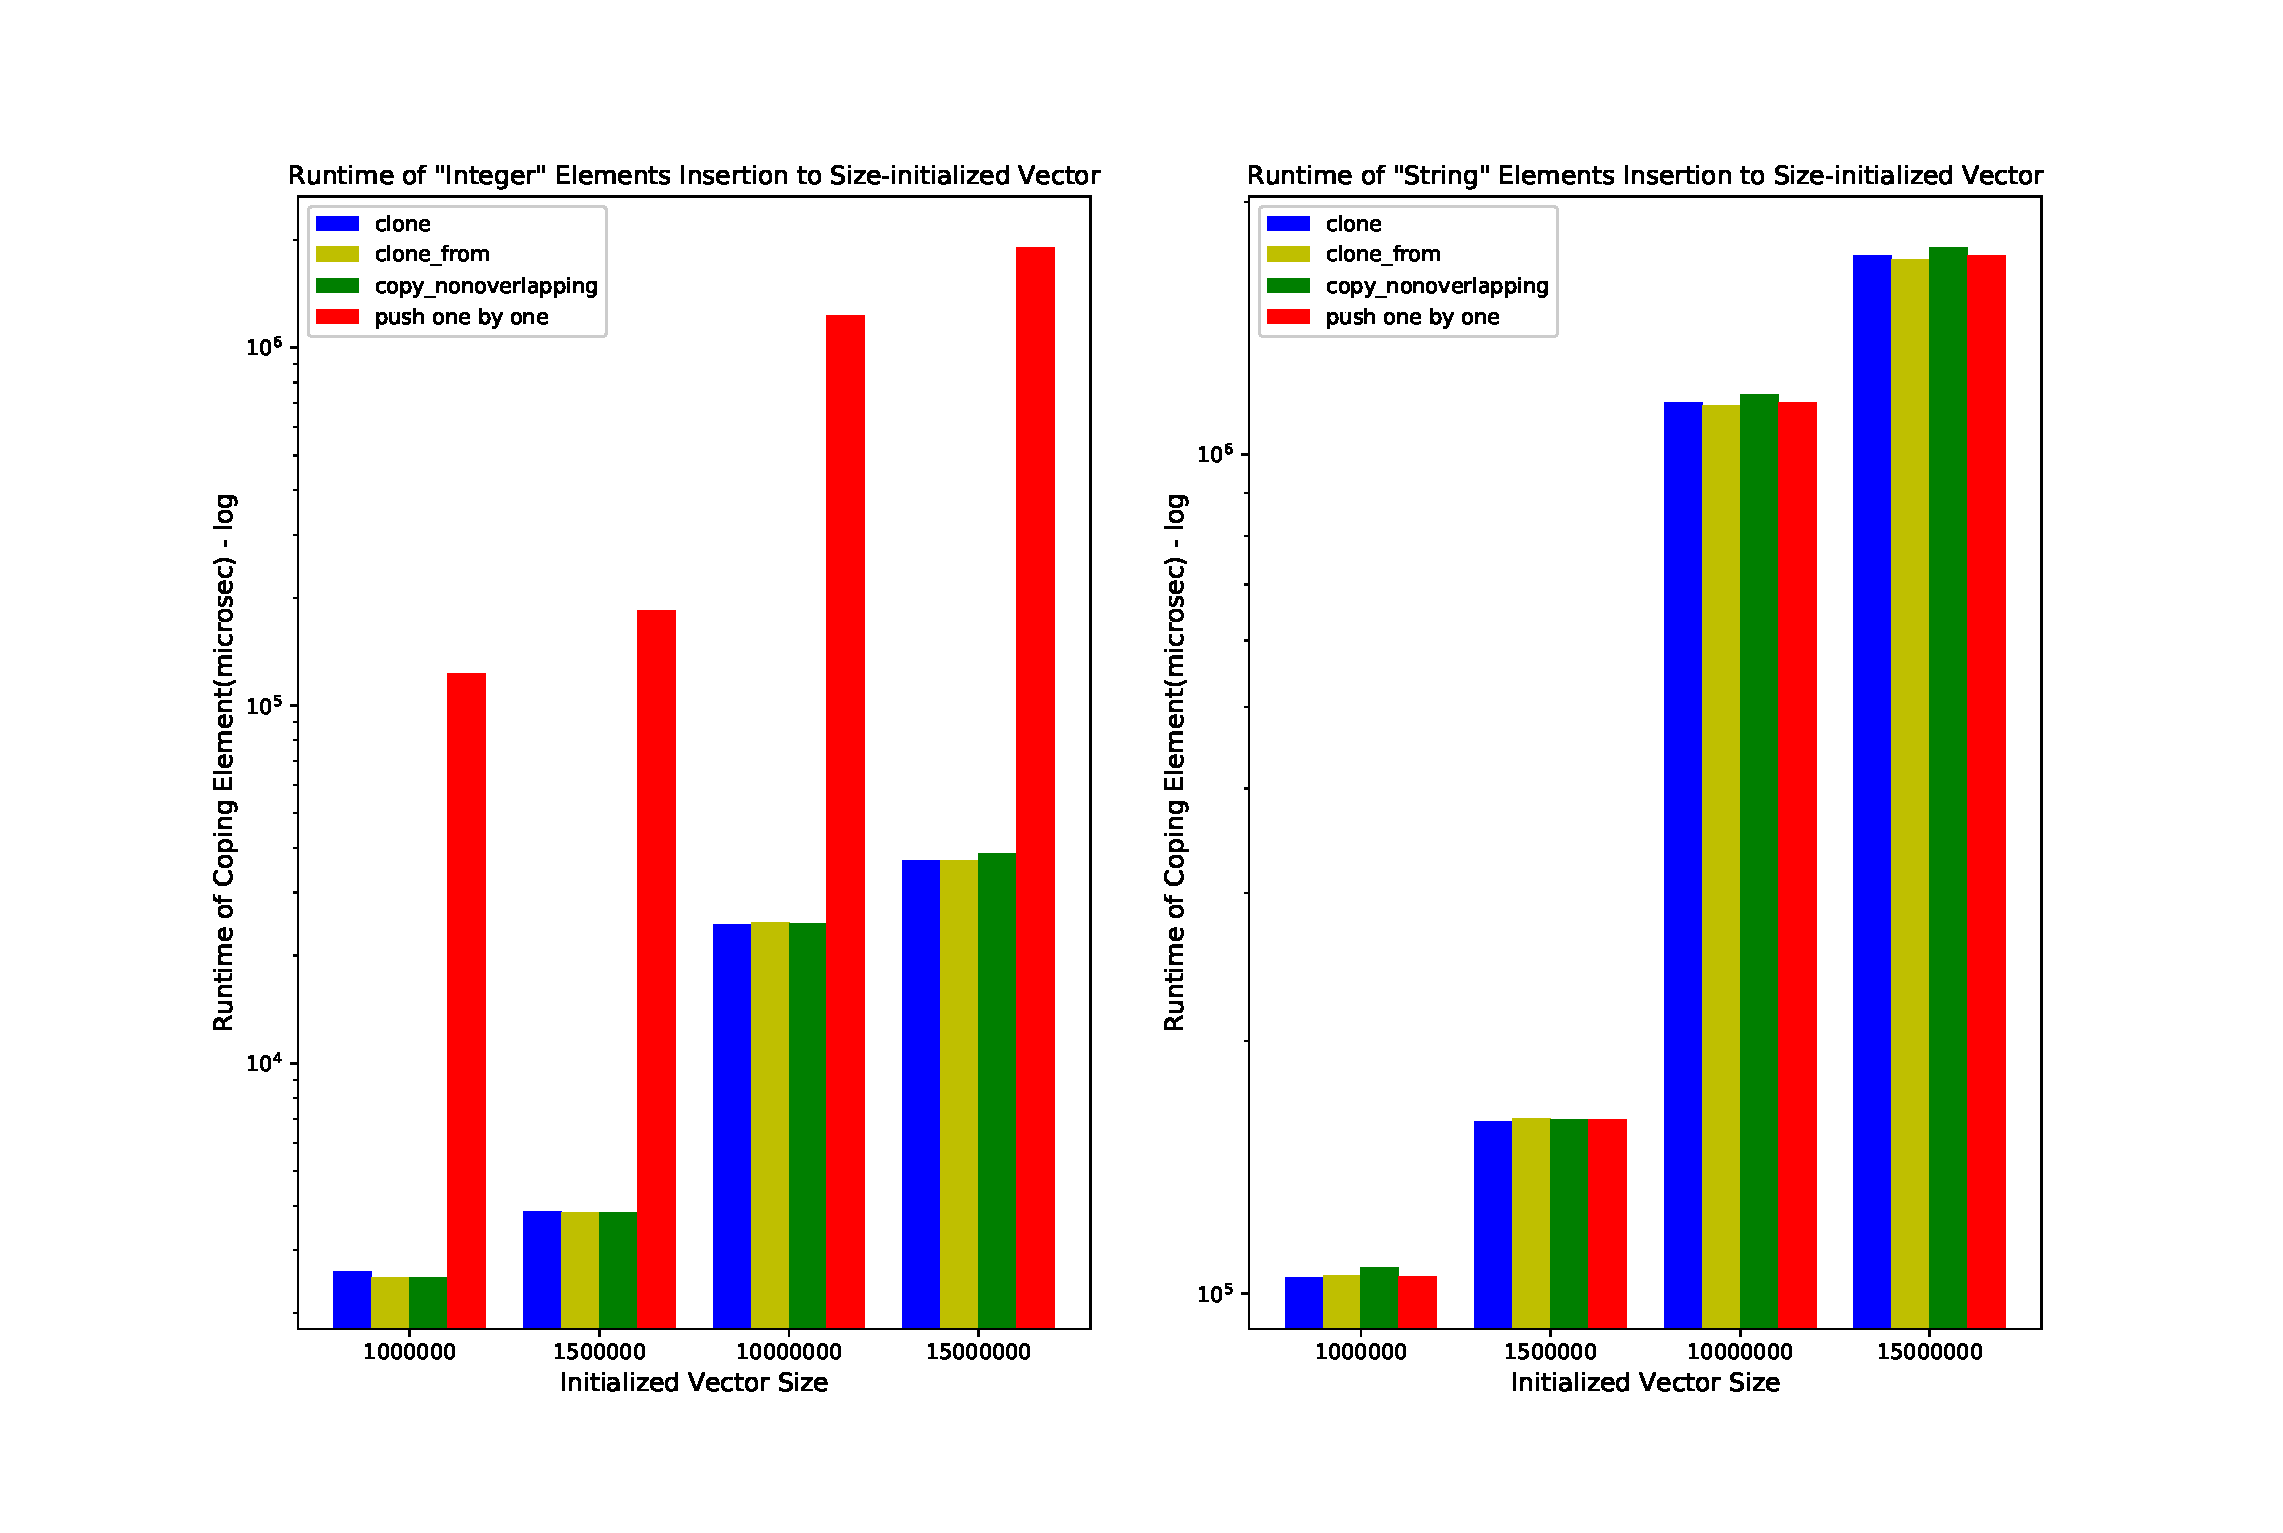
\includegraphics[width=15cm]{rust_various_insertion.eps}
    \caption{Runtime of elements copy from one vector and insertion to the other vector.}
    \label{fig:Sampling}
\end{figure}
\clearpage

\section{Access time to elements in vector}
\label{sec:history}
In this experiment, whether mutability has impacts to operation on the object in terms of runtime performance. 
According to the experiment, there is no difference on accessing to elements of mutable and immutable vector.

\begin{figure}[htb]
    \includegraphics[width=15cm]{rust_various_access.eps}
    \caption{Runtime of elements copy from one vector and insertion to the other vector.}
    \label{fig:Sampling}
\end{figure}

\section{Access time to owned, borrowed, and sliced field of object}
\label{sec:history}
In this experiment, differences of access time to among owned, borrowed, and sliced are observed. 
Each variable has slightly different use of memory. 


\begin{figure}[htb]
    \begin{lstlisting}
        struct CustomerOwned {
            key: i32,
            age: i32,
            num_purchase: i32,
            total_purchase: f64,
            duration_spent: f64, 
            duration_since: f64,
            zip_code: String,
            address: String,
            country: String,
            state: String,
            first_name: String,
            last_name: String,
            province: String,
            comment: String, 
            order: OrderOwned
        }

        struct CustomerBorrowed<'a> {
            key: &'a i32,
            age: &'a i32,
            num_purchase: &'a i32,
            total_purchase: &'a f64,
            duration_spent: &'a f64, 
            duration_since: &'a f64,
            zip_code: &'a String,
            address: &'a String,
            country: &'a String,
            state: &'a String,
            first_name: &'a String,
            last_name: &'a String,
            province: &'a String,
            comment: &'a String, 
            order: &'a OrderBorrowed<'a>
        }

        struct CustomerSlice<'a> {
            key: &'a i32,
            age: &'a i32,
            num_purchase: &'a i32,
            total_purchase: &'a f64,
            duration_spent: &'a f64, 
            duration_since: &'a f64,
            zip_code: &'a str,
            address: &'a str,
            country: &'a str, 
            state: &'a str,
            first_name: &'a str,
            last_name: &'a str,
            province: &'a str,
            comment: &'a str,
            order: &'a OrderSlice<'a>
        }

        struct CustomerRc {
            key: Rc<i32>,
            age: Rc<i32>,
            num_purchase: Rc<i32>,
            total_purchase: Rc<f64>,
            duration_spent: Rc<f64>, 
            duration_since: Rc<f64>,
            zip_code: Rc<String>,
            address: Rc<String>,
            country: Rc<String>,
            state: Rc<String>,
            first_name: Rc<String>,
            last_name: Rc<String>,
            province: Rc<String>,
            comment: Rc<String>, 
            order: Rc<OrderRc>
        }
    \end{lstlisting}
    \caption{Representation of Customer object in Rust.}
    \label{fig:Sampling}
\end{figure}

\clearpage

\begin{figure}[htb]
    \begin{lstlisting}
        struct OrderOwned {
            order_id: i32,
            num_items: i32, 
            payment: f64,
            order_time: f64,
            title: String,
            comment: String
        }


        struct OrderBorrowed<'a> {
            order_id: &'a i32,
            num_items: &'a i32, 
            payment: &'a f64,
            order_time: &'a f64,
            title: &'a String,
            comment: &'a String
        }

        struct OrderRc {
            order_id: Rc<i32>,
            num_items: Rc<i32>, 
            payment: Rc<f64>,
            order_time: Rc<f64>,
            title: Rc<String>,
            comment: Rc<String>
        }
    \end{lstlisting}
    \caption{Representation of Customer object in Rust.}
    \label{fig:Sampling}
\end{figure}
